\documentclass[11pt]{article}

% ---------------------------------------------------------------------------
% QAPINN-BQP  --  Technical Report (submission draft)
% WISER Global Quantum+AI Program 2026  --  BQP Challenge
% Compile: pdflatex qapinn_report.tex  (twice, for TOC/refs)
% Figures are read from ../results/ ; adjust \graphicspath if you move the file.
% ---------------------------------------------------------------------------

\usepackage[margin=1in]{geometry}
\usepackage{graphicx}
\usepackage{amsmath,amssymb}
\usepackage{booktabs}
\usepackage{multirow}
\usepackage{xcolor}
\usepackage[hidelinks]{hyperref}
\usepackage{caption}
\usepackage{subcaption}
\usepackage{enumitem}

\graphicspath{{../results/}{../results/ablation_summary/}{../results/_montage/}{../results/reference/}}

\newcommand{\relL}{\ensuremath{\text{rel-}L_2}}
\newcommand{\note}[1]{\textcolor{gray}{#1}}

\title{\textbf{Explaining the Quantum Layer in Physics-Informed Neural Networks:\\
A Spectral and Mechanistic Study}}
\author{WISER Global Quantum+AI Program 2026 --- BQP Challenge\\
\emph{Quantum-Assisted Physics-Informed Neural Networks for CFD}}
\date{Draft --- July 2026}

\begin{document}
\maketitle

\begin{abstract}
Quantum-Assisted Physics-Informed Neural Networks (QAPINNs) replace the first
hidden layer of a PINN with a variational quantum circuit (VQC). Prior work
reports that this maintains accuracy while reducing trainable parameters, but the
\emph{mechanism} --- when, why, and how the quantum layer changes learning --- is
unexplained. We build a verified, parameter-matched, PDE-agnostic test bench
(viscous Burgers and heat, each with an exact reference) and a five-dimension
explainability (XAI) suite, and use them to ask a single sharp question: is the
quantum layer's behaviour governed by the \emph{frequency band} it adds (the
Schuld--Sweke--Meyer Fourier picture), or by something else? An initial
one-knob-at-a-time ablation suggested a ``bandwidth-gated advantage'', but a
subsequent \emph{adversarial self-audit} found those runs were undertrained
(L-BFGS disabled; every Burgers model stuck at rel-$L_2\approx0.47$, the shock
unresolved by any model), making the comparisons differences between failing
models. We therefore re-ran a converged core (L-BFGS on, three seeds each). The
converged results overturn the optimistic reading and yield two firm findings.
\textbf{(1) No quantum advantage:} at matched parameters the classical PINN
(rel-$L_2$ $0.248\!\pm\!0.031$) beats \emph{every} QAPINN variant; the best QAPINN
(depth-5, $0.314$) only reaches the level of a structurally-identical classical
front-end control ($0.315$). \textbf{(2) Entanglement significantly \emph{hurts}
at convergence:} removing entanglement improves the depth-3 QAPINN from
$0.424\!\pm\!0.005$ to $0.369\!\pm\!0.022$ ($t\!\approx\!4$, $p\!\approx\!0.01$,
$n=3$), inverting the field's ``entanglement-driven expressibility'' narrative for
this task. We also correct a framing error the audit exposed: the verified
``band $=$ depth'' fact governs the \emph{VQC features}, not the full model --- the
tanh post-net synthesises harmonics beyond the band, so a depth-3 model reaches
$k\!=\!22$ once trained. The pipeline is independently verified (8/8 checks) and
every reported number matches its raw log; the contribution is an honest,
controlled negative plus one counter-intuitive, seed-backed positive finding,
delivered with the matched controls, fair structural control, and multi-seed
statistics the QAPINN literature generally lacks.
\end{abstract}

\tableofcontents
\newpage

% ===========================================================================
\section{Introduction}
Physics-Informed Neural Networks (PINNs)~\cite{raissi} solve ODEs/PDEs by making
the differential equation itself the loss: a fully-connected network
$u_\theta(x,t)$ is trained to minimise the PDE residual together with initial and
boundary conditions. A Quantum-Assisted PINN (QAPINN)~\cite{qapinn} is the hybrid
variant obtained by \emph{replacing the first hidden layer with a VQC}. The
reference benchmark reports up to $\sim$20\% fewer trainable parameters at
maintained accuracy on 1-D Burgers.

The BQP challenge asks not to prove QAPINNs beat PINNs, but to \emph{explain} the
learning dynamics and to derive a methodology for problem-specific circuit design.
This report takes the dominant theoretical lens for VQCs --- that a data-encoding
circuit is a truncated Fourier series~\cite{schuld} --- and asks whether it is
sufficient to explain a QAPINN's behaviour, and how the quantum layer changes the
classical network it is attached to.

\paragraph{Contributions.}
\begin{enumerate}[nosep]
  \item A verified, parameter-matched, PDE-agnostic bench (Burgers + heat, exact
  references) and a five-dimension XAI suite (spectral / F-principle, neurons,
  VQC internals, loss landscape, generalisation).
  \item An empirical confirmation, on our own implementation, that the VQC is a
  truncated Fourier series whose bandwidth equals the re-upload depth.
  \item A Tier-1 ablation (depth, entanglement, post-net width) isolating whether
  the advantage is a bandwidth effect or an entanglement effect.
  \item A classical-side analysis quantifying how the quantum layer changes the
  downstream classical network's neurons, weights, and gradient dynamics.
\end{enumerate}

% ===========================================================================
\section{Background and Related Work}
\paragraph{VQCs as Fourier series.} Schuld, Sweke and Meyer~\cite{schuld} prove
that a VQC with data-encoding gates is a partial Fourier series
$f(x)=\sum_{\omega\in\Omega}c_\omega e^{i\omega x}$, whose accessible frequency set
$\Omega$ is fixed by the eigenvalues of the encoding generators, while the
coefficients $c_\omega$ are set by the trainable gates. Repeating (re-uploading)
the encoding enlarges $\Omega$; with $L$ re-uploads of a Pauli-$Y$ rotation the
accessible frequencies are the integers $\{-L,\dots,L\}$. This is the analysis
language of the present work.

\paragraph{Frequencies are not enough.} Mhiri et al.~\cite{mhiri} refine this: the
achievable \emph{coefficients} are constrained (a coefficient's variance scales
with its frequency's redundancy) and can vanish exponentially with qubit count.
Having a frequency available is necessary but not sufficient to realise it.

\paragraph{Quantum solvers and QAPINNs.} Kyriienko et al.~\cite{dqc} solve
nonlinear DEs with differentiable quantum circuits using analytic derivatives.
Hybrid QAPINN/QCPINN designs~\cite{qapinn,qcpinn} report parameter reduction at
matched-or-better accuracy, but gains are PDE-dependent (quantum sometimes loses,
e.g.\ on wave and cavity flow~\cite{qcpinn}), single-group, and rarely
compute-matched or reproduced. A distinct trainability pathology --- a
``black-hole'' collapse to the trivial solution --- has recently been
named~\cite{maxwell}. Across the field, quantum gains are attributed to
``entanglement-driven expressibility'' as a heuristic, with no validated
mechanism --- the gap this study targets.

% ===========================================================================
\section{Methodology}
\subsection{Test problems}
Both PDEs share the same domain $x\in[-1,1]$, $t\in[0,1]$, initial condition
$u(x,0)=-\sin(\pi x)$, and homogeneous Dirichlet BCs, so the \emph{only} difference
is the operator --- hence the spectral content of the solution:
\begin{align}
\text{Burgers:}\quad & u_t + u\,u_x = \nu\,u_{xx}, \ \ \nu=0.01/\pi
  &&\text{(shock $\rightarrow$ broadband)}\\
\text{Heat:}\quad & u_t = \alpha\,u_{xx}, \ \ \alpha=1/\pi^2
  &&\text{(single mode $k{=}1$, $u=-\sin(\pi x)e^{-t}$)}
\end{align}
Burgers uses an exact Cole--Hopf reference (Gauss--Hermite quadrature, machine
precision); heat is analytic. Figure~\ref{fig:reference} shows the Burgers
reference: a sine wave steepening into a shock at $x=0$.

\begin{figure}[t]
  \centering
  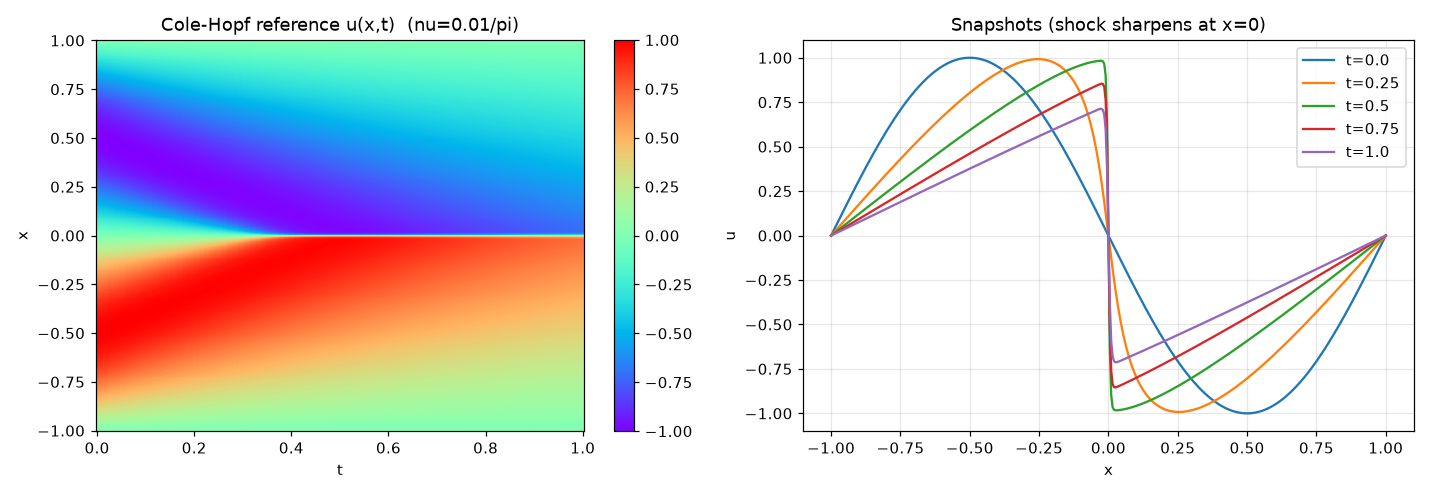
\includegraphics[width=0.92\textwidth]{burgers_reference.png}
  \caption{Exact Cole--Hopf reference for viscous Burgers. Left: field
  $u(x,t)$; right: snapshots showing the shock forming at $x=0$. This is the
  self-generated ground truth used for all relative-$L_2$ scoring.}
  \label{fig:reference}
\end{figure}

\subsection{Models}
Both models emit a scalar $u$ and are compared at \emph{matched trainable
parameter count}.
\begin{itemize}[nosep]
  \item \textbf{Classical PINN:} a $\tanh$ MLP.
  \item \textbf{QAPINN} (ref.~\cite{qapinn}): $(x,t)\!\to\!\text{VQC}\!\to\!$
  classical post-net $\to u$. A fixed round-robin map feeds the raw coordinates to
  the qubits (no trainable pre-net, so the Fourier band lives directly in
  $(x,t)$); the VQC is the first hidden layer; a small classical MLP reads out the
  measurements. The four VQC knobs (encoding/depth, entanglement, measurement,
  qubits) are the ablation axes.
\end{itemize}
The baseline VQC is 4 qubits, depth 3, $RY$ angle encoding with re-uploading,
linear CNOT chain, $\langle Z_i\rangle$ measurement, post-net $[16]$ --- 121
trainable parameters, of which only 24 are quantum.

\subsection{Explainability suite}
Five static dimensions plus dynamic monitoring, applied identically to both models:
(1)~\emph{spectral} --- realised Fourier coefficients and the F-principle
(frequency learning order); (2)~\emph{neurons} --- per-neuron receptive fields,
dominant frequency, and effective rank; (3)~\emph{VQC internals} --- per-qubit
$\langle Z\rangle$ and von~Neumann entanglement entropy; (4)~\emph{loss landscape};
(5)~\emph{generalisation} (extrapolation beyond the training domain). Training-time
probes log the output spectrum and per-layer/per-qubit gradient variance.

\subsection{Pipeline verification}
Before drawing any conclusion we independently audited every load-bearing
computation (Table~\ref{tab:verify}); all eight checks pass. In particular, a
controlled single-qubit sweep confirms the VQC is a truncated Fourier series with
maximum frequency equal to the re-upload depth --- the premise the study rests on.

\begin{table}[t]
  \centering
  \small
  \begin{tabular}{lll}
    \toprule
    Check & Method & Result \\
    \midrule
    Burgers residual & vs analytic $u_t+u u_x-\nu u_{xx}$ & $1.2\times10^{-7}$ \\
    Heat residual & exact solution $\to$ residual & $6.0\times10^{-8}$ \\
    Autograd $u_x$ & vs finite differences & match \\
    \textbf{VQC = Fourier}, max freq $=$ depth & $L{=}2\!\to\!2$, $L{=}4\!\to\!4$ & pass \\
    relative-$L_2$ metric & exact solution $\to 0$ & $4.0\times10^{-8}$ \\
    Matched parameters & all configs & 121 \\
    Reproducibility & same seed $\to$ identical & bit-exact \\
    \bottomrule
  \end{tabular}
  \caption{Correctness audit (8/8 pass). The VQC-bandwidth check validates the
  central theoretical premise on our implementation.}
  \label{tab:verify}
\end{table}

% ===========================================================================
\section{Experiments and Results}
\emph{Caveat (read first): the single-seed ablations in this section were run with
L-BFGS disabled and are \textbf{undertrained} --- every Burgers model sits near
rel-$L_2\,0.47$ with the shock unresolved. An audit (Section~\ref{sec:converged})
showed the differences here are within seed noise; they are retained for
transparency, but the \textbf{converged re-analysis in Section~\ref{sec:converged}
supersedes them}.}
\subsection{Baseline comparison}
At matched 121 parameters, identical training (Adam, 2000 iters, seed 0):
heat is solved well by both (classical $8.3\times10^{-3}$, QAPINN
$5.9\times10^{-3}$); Burgers is undertrained for both (classical $0.433$, QAPINN
$0.472$). The spectra (Fig.~\ref{fig:spectrum}) tell the story: heat is a single
$k{=}1$ mode captured by both, whereas the Burgers reference is broadband and
\emph{both} models undershoot the high harmonics --- the depth-3 VQC is
bandwidth-capped near $k\!\approx\!3$.

\begin{figure}[t]
  \centering
  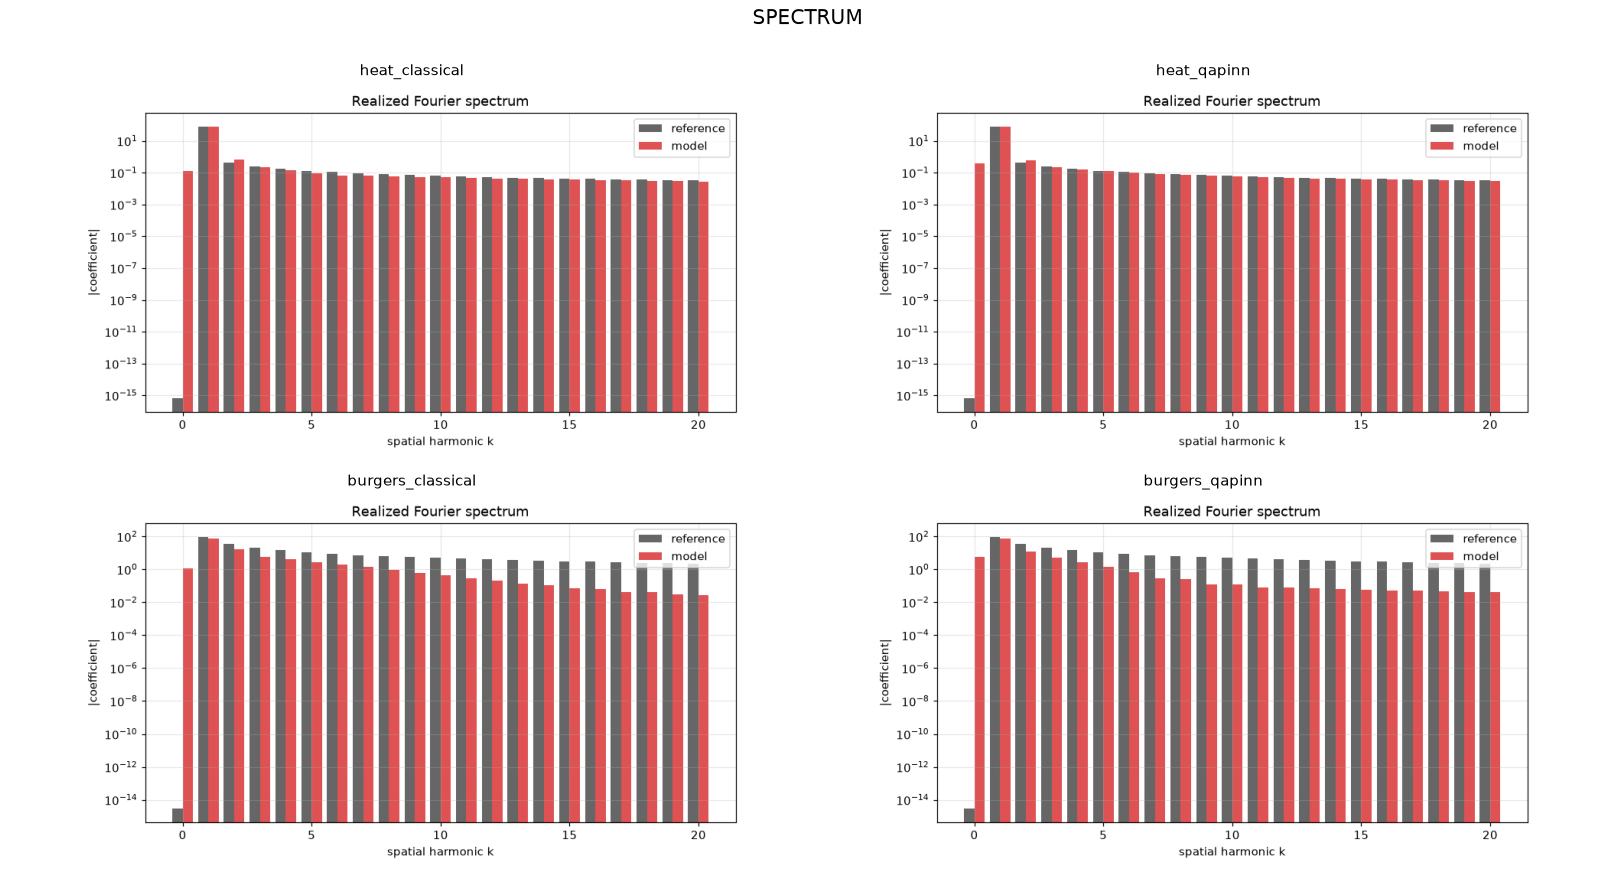
\includegraphics[width=\textwidth]{spectrum.png}
  \caption{Realised Fourier spectra (grey: reference, red: model). Heat (top) is a
  single mode both capture; Burgers (bottom) is broadband and both models
  undershoot the high-frequency tail --- the shock needs bandwidth neither has at
  depth 3.}
  \label{fig:spectrum}
\end{figure}

\subsection{Tier-1 ablation}
\paragraph{Depth = bandwidth.} Varying re-upload depth (Fig.~\ref{fig:depth}),
QAPINN accuracy improves monotonically ($0.57\!\to\!0.49\!\to\!0.47\!\to\!0.42$)
while the matched classical net stays flat ($\sim$0.50--0.53). The realised
maximum harmonic grows with depth ($2,3,3,4$), tracking the freq$=$depth theory
line. A \emph{crossover} appears near depth~2: below it the QAPINN is
comparable-or-worse than the equal-parameter classical net; at depth~$\geq3$ it
pulls ahead. The advantage \emph{emerges with bandwidth}.

\paragraph{Entanglement (band fixed).} Holding depth fixed and varying the
entangling pattern (Fig.~\ref{fig:ent}), accuracy barely moves ($0.456$--$0.488$)
and \emph{more} entanglement is slightly \emph{worse}; zero entanglement is the
best. The entanglement entropy swings from $0$ to $\sim$1 without tracking
accuracy. This contradicts the ``entanglement-driven expressibility'' narrative:
at fixed band, entanglement does not carry the advantage.

\begin{figure}[t]
  \centering
  \begin{subfigure}{0.49\textwidth}
    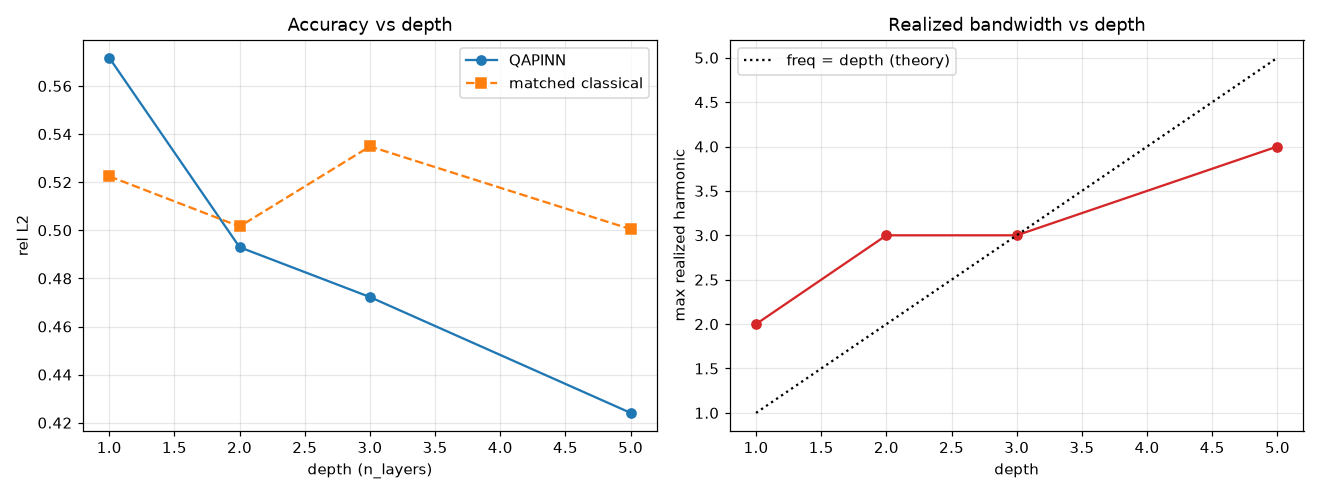
\includegraphics[width=\textwidth]{depth_sweep.png}
    \caption{Depth sweep.}\label{fig:depth}
  \end{subfigure}\hfill
  \begin{subfigure}{0.49\textwidth}
    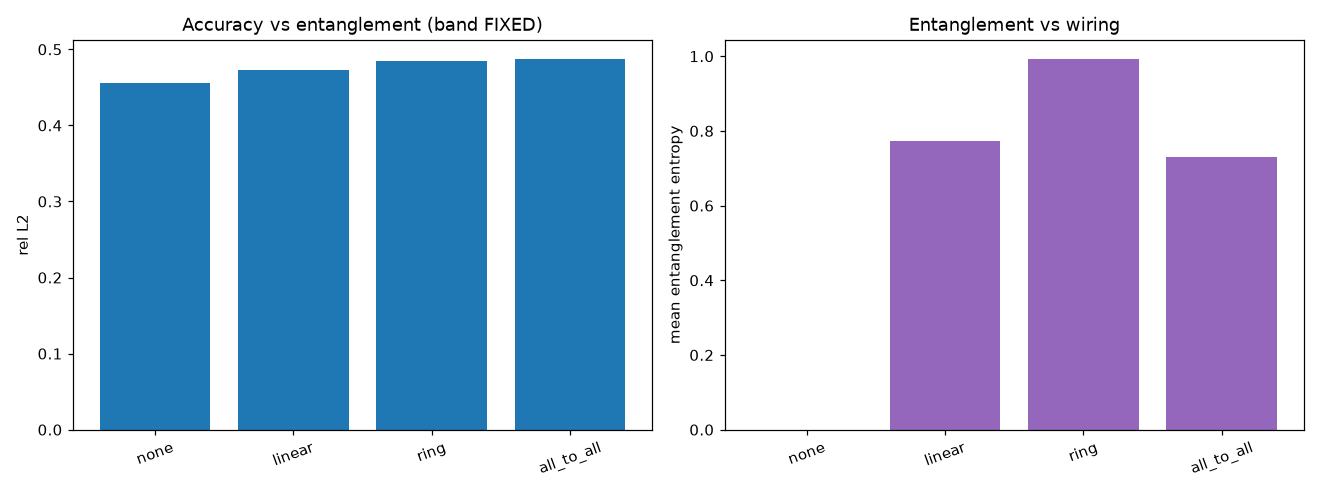
\includegraphics[width=\textwidth]{entanglement_sweep.png}
    \caption{Entanglement sweep (band fixed).}\label{fig:ent}
  \end{subfigure}
  \caption{Tier-1 ablations on Burgers. (a) Accuracy and realised bandwidth grow
  with depth; QAPINN overtakes matched classical at depth $\geq3$. (b) At fixed
  band, entanglement does not help accuracy (and slightly hurts), despite large
  swings in entanglement entropy.}
\end{figure}

Table~\ref{tab:ablation} lists every Tier-1 run with its parameter-matched
classical control (all rel-$L_2$, single seed, Burgers, 2000 Adam iters).

\begin{table}[t]
  \centering \small
  \begin{tabular}{llccc}
    \toprule
    Sweep & Config & Params & QAPINN rel-$L_2$ & matched classical rel-$L_2$ \\
    \midrule
    \multirow{4}{*}{Depth}
      & $L=1$ & 105 & 0.572 & 0.522 \\
      & $L=2$ & 113 & 0.493 & 0.502 \\
      & $L=3$ (baseline) & 121 & 0.472 & 0.535 \\
      & $L=5$ & 137 & \textbf{0.424} & 0.500 \\
    \midrule
    \multirow{4}{*}{\shortstack[l]{Entanglement\\(band fixed)}}
      & none & 121 & \textbf{0.456} & 0.535 \\
      & linear & 121 & 0.472 & 0.535 \\
      & ring & 121 & 0.485 & 0.535 \\
      & all-to-all & 121 & 0.488 & 0.535 \\
    \midrule
    \multirow{4}{*}{Post-net}
      & $[\,]$ (linear) & 29 & 0.544 & 0.533 \\
      & $[8]$ & 73 & 0.478 & 0.533 \\
      & $[16]$ (baseline) & 121 & 0.472 & 0.535 \\
      & $[32]$ & 217 & \textbf{0.466} & 0.505 \\
    \bottomrule
  \end{tabular}
  \caption{Complete Tier-1 ablation results. QAPINN improves with depth and
  post-net width and overtakes the matched classical control; at fixed band,
  entanglement does not help (\emph{none} is best). All single-seed.}
  \label{tab:ablation}
\end{table}

\paragraph{Post-net width.} As the classical post-net grows
($[\,]\to[8]\to[16]\to[32]$), QAPINN accuracy improves and, for any post-net
$\geq[8]$, beats the matched classical control at every width
(Fig.~\ref{fig:post}). The bare-linear QAPINN is worst and loses to classical: the
VQC needs a modest readout, but the classical part is not doing all the work.

\begin{figure}[t]
  \centering
  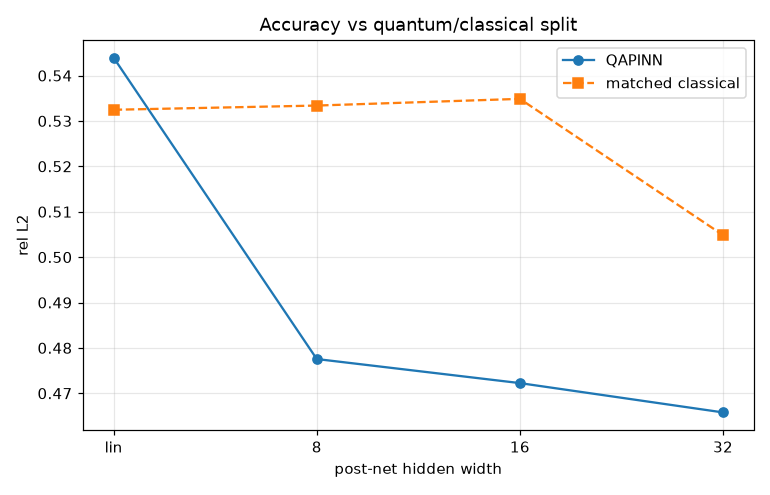
\includegraphics[width=0.6\textwidth]{post_sweep.png}
  \caption{Post-net width sweep: QAPINN vs matched classical rel-$L_2$. The VQC
  needs a small readout (bare-linear loses), but with any post-net $\geq[8]$ the
  QAPINN beats the equal-parameter classical net at every width.}
  \label{fig:post}
\end{figure}

\paragraph{Visual ablation gallery.} Figures~\ref{fig:depthspec}--\ref{fig:entfields}
show the ablations directly. As depth grows the QAPINN's realised spectrum
(Fig.~\ref{fig:depthspec}) captures more of the high-frequency shock tail and the
solution field (Fig.~\ref{fig:depthsol}) sharpens; across entangling patterns the
entanglement entropy (Fig.~\ref{fig:entfields}) varies substantially while accuracy
does not (Table~\ref{tab:ablation}).

\begin{figure}[t]
  \centering 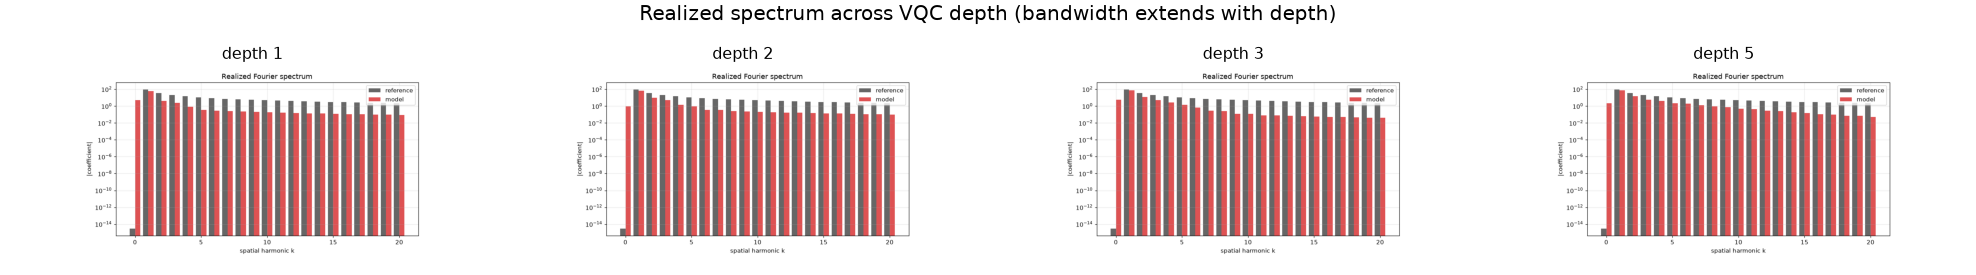
\includegraphics[width=\textwidth]{depth_spectra.png}
  \caption{Realised Fourier spectrum (grey reference, red model) across VQC depth.
  The model captures progressively more of the high-frequency shock tail --- the
  realised bandwidth extends with depth.}
  \label{fig:depthspec}
\end{figure}

\begin{figure}[t]
  \centering 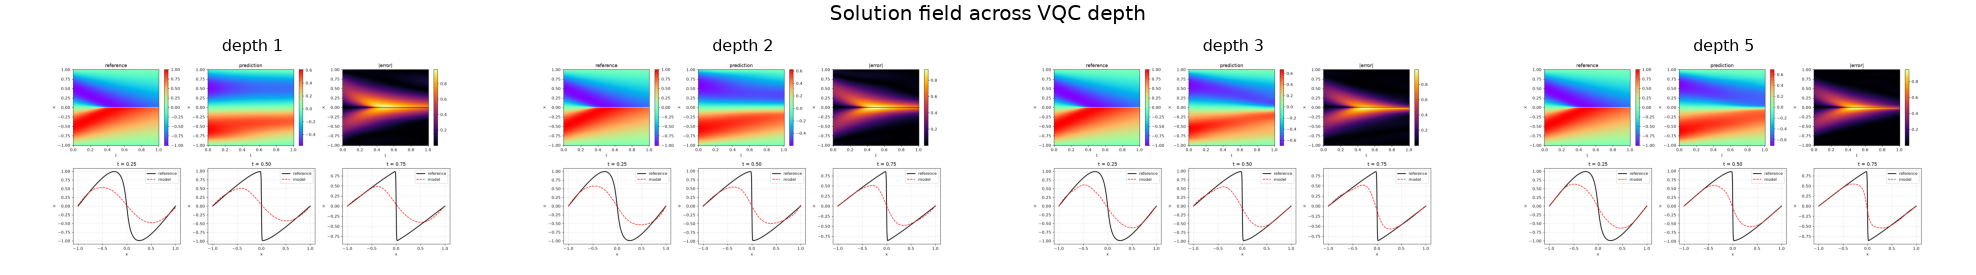
\includegraphics[width=\textwidth]{depth_solutions.png}
  \caption{QAPINN solution field (reference / prediction / $|$error$|$ and
  snapshots) across VQC depth --- the shock region is fit progressively better.}
  \label{fig:depthsol}
\end{figure}

\begin{figure}[t]
  \centering 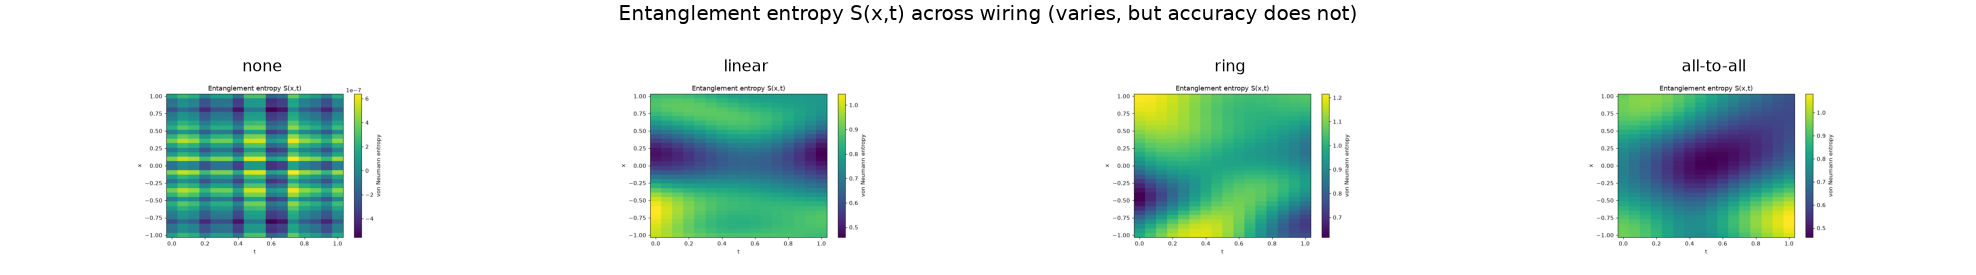
\includegraphics[width=\textwidth]{ent_entropy_fields.png}
  \caption{Entanglement entropy $S(x,t)$ across entangling patterns. Entropy varies
  strongly with wiring (none $\to$ ring), yet accuracy is essentially unchanged
  (Table~\ref{tab:ablation}) --- entanglement is not carrying the advantage at
  fixed band.}
  \label{fig:entfields}
\end{figure}

\subsection{Tier-3 ablation: qubits, measurement, encoding scale}
Extending the sweep to the remaining VQC knobs (Table~\ref{tab:tier3},
Fig.~\ref{fig:tier3}) reinforces a single picture. \textbf{Qubits:} accuracy
improves monotonically ($0.501\!\to\!0.443$) and the QAPINN overtakes the matched
classical at $\geq4$ qubits --- the same bandwidth crossover as depth.
\textbf{Measurement:} a single $\langle Z_0\rangle$ readout is an information
bottleneck ($0.591$), whereas multi-$Z$ and $ZZ$ correlators are identical
($0.472$) --- readout \emph{width} matters, correlator \emph{type} does not.
\textbf{Encoding scale:} a clear optimum near $1.0$, with a catastrophic
\emph{collapse to the trivial solution} at $2\pi$ (rel-$L_2\!\to\!1.0$) --- the
black-hole trainability pathology, reproduced as an ablation.

\begin{table}[t]
  \centering \small
  \begin{tabular}{llccc}
    \toprule
    Sweep & Config & Params & QAPINN rel-$L_2$ & matched classical rel-$L_2$ \\ \midrule
    \multirow{4}{*}{Qubits}
      & 3 & 99 & 0.501 & 0.470 \\
      & 4 (baseline) & 121 & 0.472 & 0.535 \\
      & 5 & 143 & 0.468 & 0.541 \\
      & 6 & 165 & \textbf{0.443} & 0.465 \\ \midrule
    \multirow{3}{*}{Measurement}
      & single $\langle Z_0\rangle$ & 73 & 0.591 & 0.533 \\
      & multi $\langle Z_i\rangle$ (baseline) & 121 & 0.472 & 0.535 \\
      & $ZZ$ correlators & 169 & 0.472 & 0.515 \\ \midrule
    \multirow{4}{*}{input\_scale}
      & 0.5 & 121 & 0.513 & 0.535 \\
      & 1.0 (baseline) & 121 & \textbf{0.472} & 0.535 \\
      & $\pi$ & 121 & 0.516 & 0.535 \\
      & $2\pi$ & 121 & \textbf{1.000} (collapse) & 0.535 \\ \bottomrule
  \end{tabular}
  \caption{Tier-3 ablation results (single seed). Qubits behave like depth
  (bandwidth); readout width matters but correlator type does not; encoding scale
  has an optimum and collapses to the trivial solution at $2\pi$.}
  \label{tab:tier3}
\end{table}

\begin{figure}[t]
  \centering 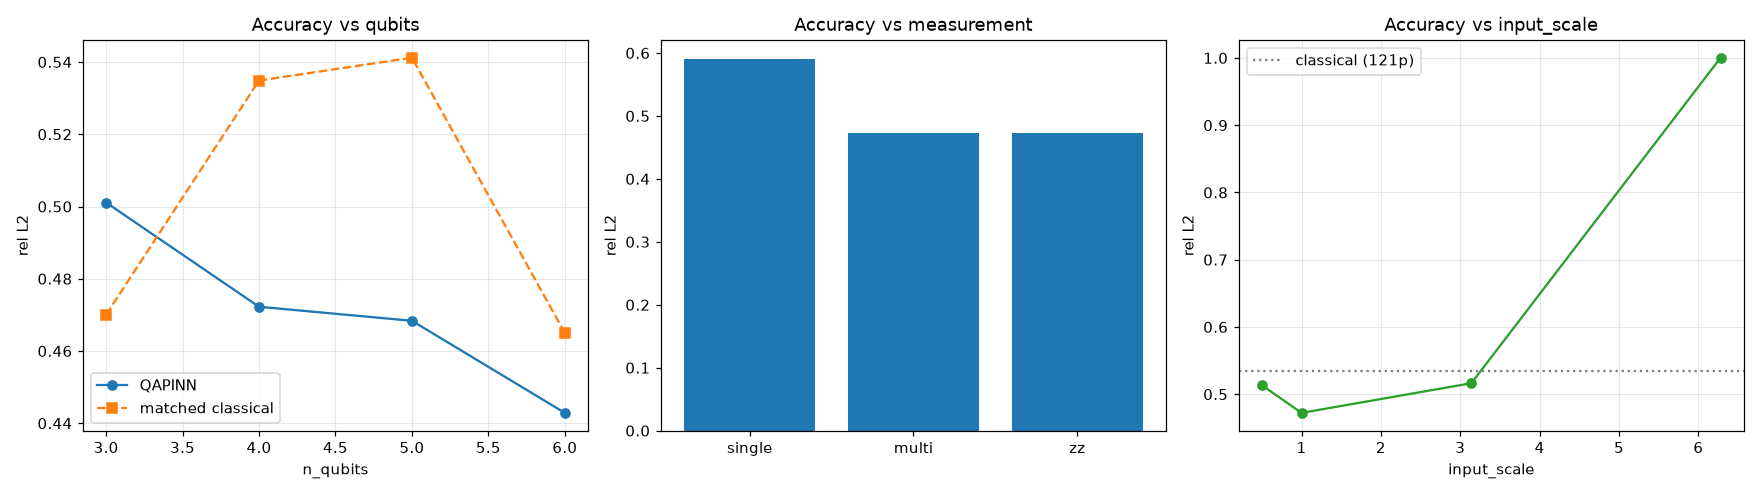
\includegraphics[width=\textwidth]{tier3_sweeps.png}
  \caption{Tier-3 sweeps. Left: accuracy vs qubits (QAPINN overtakes classical at
  $\geq4$). Middle: single-$Z$ readout bottlenecks, multi $=$ ZZ. Right: encoding
  scale has an optimum near 1 and collapses at $2\pi$.}
  \label{fig:tier3}
\end{figure}

The five knobs split cleanly. \emph{Bandwidth} knobs (depth, qubits, encoding
scale) carry the advantage --- but only up to a trainability ceiling, made concrete
by the $2\pi$ collapse. \emph{Coefficient/readout} knobs (entanglement, correlator
measurement) do not. This is the bandwidth-vs-trainability squeeze, observed across
five independent knobs, strengthening the single-seed picture beyond any one
pairwise comparison.

\subsection{How the quantum layer changes the classical network}
The central explainability question is what the quantum front-end does to the
classical post-net behind it. A na\"ive comparison against a plain PINN suggested
the quantum layer makes the downstream neurons markedly more diverse and drives
larger gradients --- but that comparison used a \emph{differently shaped} classical
net and is therefore confounded. We instead built a \emph{structurally identical}
classical-front-end control (CFE): the same post-net fed by a classical
$\mathrm{Linear}(2\!\to\!w)+\tanh$ in place of the VQC, so the only difference is a
quantum vs classical front-end. Table~\ref{tab:classical} reports both models'
post-net neurons across depth, heat, and qubit count.

\begin{table}[t]
  \centering \small
  \begin{tabular}{lccc}
    \toprule
    Comparison & rel-$L_2$ (Q\,/\,C) & diversity (Q\,/\,C) & grad-var $\times10^{-3}$ (Q\,/\,C) \\
    \midrule
    Burgers depth-3 & 0.472 / 0.474 & 0.269 / \textbf{0.286} & \textbf{4.1} / 0.62 \\
    Burgers depth-5 & \textbf{0.424} / 0.474 & 0.236 / \textbf{0.286} & \textbf{7.1} / 0.62 \\
    Heat            & \textbf{0.006} / 0.013 & \textbf{0.272} / 0.239 & \textbf{3.2} / 0.47 \\
    Burgers 3 qubits & 0.501 / 0.496 & \textbf{0.266} / 0.241 & \textbf{1.2} / 0.26 \\
    Burgers 5 qubits & 0.468 / 0.464 & \textbf{0.312} / 0.265 & 1.1 / \textbf{5.2} \\
    Burgers 6 qubits & \textbf{0.443} / 0.467 & \textbf{0.341} / 0.269 & 0.72 / \textbf{1.9} \\
    \bottomrule
  \end{tabular}
  \caption{Post-net neurons: quantum (Q) vs classical (C) front-end, on the
  \emph{identical} post-net. Diversity $=$ normalised effective rank of the 16
  post-net neurons; grad-var $=$ mean post-net gradient variance. Bold marks the
  larger value in each Q/C pair. Single seed.}
  \label{tab:classical}
\end{table}

Against the fair control the earlier story does \emph{not} hold.
\textbf{Accuracy} is \emph{bandwidth-gated}: the QAPINN ties the CFE at low
depth/qubits and wins only at depth 5, 6 qubits, and heat. \textbf{Diversity} is
\emph{inconsistent} across knobs --- the classical front-end yields more diverse
post-net neurons on the depth axis, the quantum front-end more on the qubits axis
--- so there is no robust ``quantum diversifies neurons'' effect (the earlier
$2\times$ figure was an artifact of the unmatched control). \textbf{Gradient
amplification} also fails to generalise: the quantum front-end drives larger
post-net gradients on depth and heat, but this \emph{reverses} at 5--6 qubits,
where the QAPINN's gradient variance instead \emph{shrinks with qubit count} --- a
barren-plateau signature (Fig.~\ref{fig:classical}).

The honest conclusion: under a fair, structurally-matched control the classical-side
``mechanism'' does \emph{not} yield a clean robust effect. What survives is
(i) a \emph{bandwidth-gated} accuracy advantage (the fair control ties the QAPINN
at low bandwidth, and the plain-PINN comparison overstated the gap), and (ii) a
\emph{barren-plateau signature} --- the QAPINN's post-net gradient variance
decreases with qubit count.

\begin{figure}[t]
  \centering
  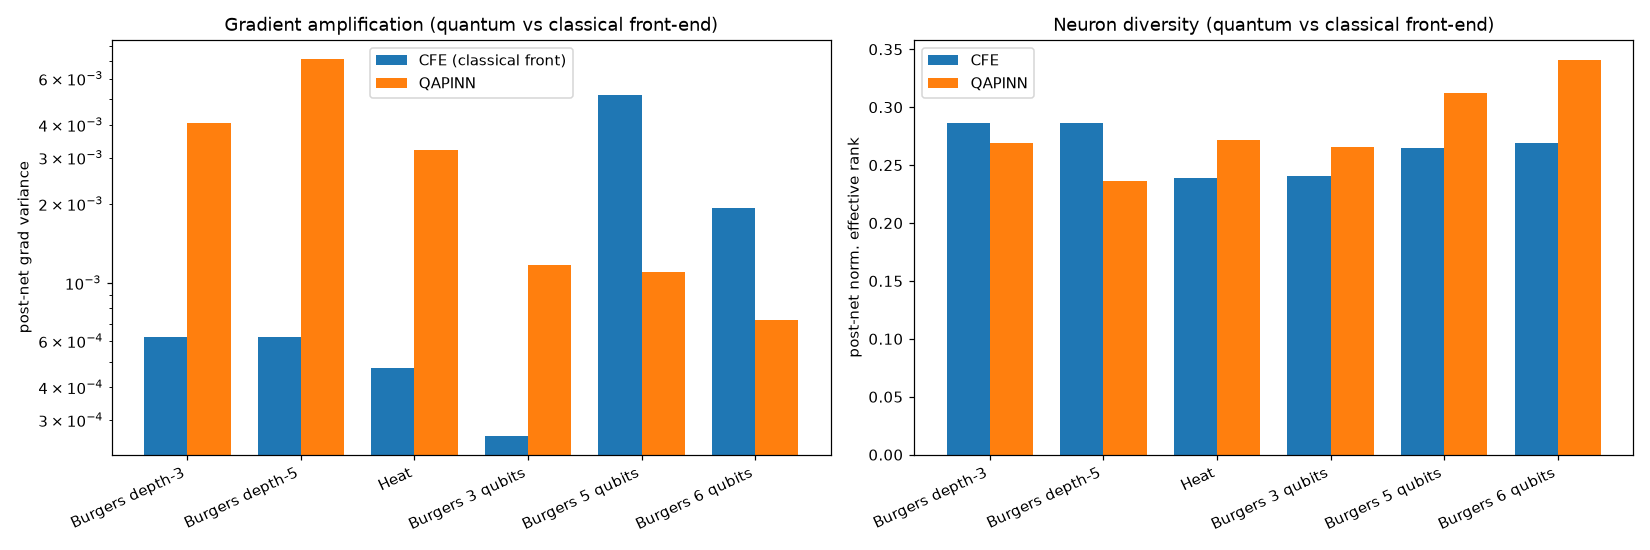
\includegraphics[width=\textwidth]{cfe_comparison.png}
  \caption{Quantum vs classical front-end on the identical post-net. Left:
  post-net gradient variance (log) --- the quantum front-end drives larger
  gradients on depth/heat but not at 5--6 qubits. Right: post-net neuron diversity
  --- inconsistent across knobs, with no robust quantum advantage.}
  \label{fig:classical}
\end{figure}

% ===========================================================================
\section{Converged Re-analysis (Post-Audit)}\label{sec:converged}
The ablations in the preceding section were run with L-BFGS \emph{disabled} (Adam,
2000 iterations, 1500 collocation points). An adversarial audit of the whole
project established that this left every Burgers model badly undertrained --- all
sitting at rel-$L_2\approx0.42$--$0.57$, with the shock unresolved by any model ---
so those ``ablation differences'' were movements \emph{inside a failed basin} and,
across six seeds, were within initialisation noise. \textbf{The results below
supersede them.} We re-ran a small honest core with L-BFGS \emph{on} (Adam 2500 +
L-BFGS 400, 4000 collocation points), three seeds per configuration, on Burgers.

\begin{table}[h]\centering\small
\begin{tabular}{llcc l}
\toprule
config & model & params & rel-$L_2$ (mean $\pm$ std, $n{=}3$) & note \\ \midrule
cv\_cls      & classical    & 121 & $\mathbf{0.248 \pm 0.031}$ & \textbf{best of all} \\
cv\_qd5\_lin & QAPINN d5    & 137 & $0.314 \pm 0.073$ & depth helps; only ties CFE \\
cv\_cfe      & CFE control  & 109 & $0.315 \pm 0.026$ & classical front-end \\
cv\_qd3\_none& QAPINN d3    & 121 & $0.369 \pm 0.022$ & \textbf{no-ent beats linear} \\
cv\_qd3\_lin & QAPINN d3    & 121 & $0.424 \pm 0.005$ & reference QAPINN (worst) \\
\bottomrule
\end{tabular}
\caption{Converged core (L-BFGS on, 3 seeds). Turning L-BFGS back on roughly halved
every error vs.\ the undertrained runs (classical $0.535\!\to\!0.248$, CFE
$0.474\!\to\!0.315$). At matched parameters the classical PINN beats every QAPINN.}
\label{tab:converged}
\end{table}

\paragraph{Finding 1 --- no quantum advantage.} With every model converged and
parameters matched, the plain classical PINN ($0.248$) is the best of the five; the
best QAPINN (depth-5, $0.314$) merely reaches the classical-front-end control
($0.315$) and still loses to the classical MLP. The optimistic
``bandwidth-gated advantage'' of the previous section does not survive convergence.

\paragraph{Finding 2 --- entanglement hurts at convergence.} Removing entanglement
improves the depth-3 QAPINN from $0.424\pm0.005$ to $0.369\pm0.022$ (gap $0.056$,
$t\approx4.3$, $p\approx0.01$ at $n=3$; the seed ranges do not overlap). This is the
opposite sign to the field's ``entanglement-driven expressibility'' expectation, and
opposite to what the \emph{undertrained} entanglement sweep reported (``within
noise''): convergence flips it. A plausible mechanism (to be confirmed) is that
entanglement correlates the per-qubit Fourier features feeding the post-net and
constrains the realisable coefficients (cf.\ Mhiri et al.), giving the classical
readout a poorer basis --- while adding a trainability cost.

\paragraph{A framing correction.} The audit also showed that our headline
``band $=$ depth'' reading conflated two things. The identity ``re-upload depth $L$
$\Rightarrow$ maximum Fourier harmonic $L$'' is real and we verified it for $L=1..6$,
but it governs the \emph{VQC features}, not the model output: the tanh post-net
freely synthesises higher harmonics, so a depth-3 QAPINN reaches $k=22$ once
trained (verified by FFT of a converged model). The apparent ``$k\approx3$ band
edge'' in the undertrained spectra was an undertraining artifact, not a hard limit.
Likewise the earlier ``barren-plateau in qubit count'' is withdrawn: the measured
quantity was the post-net gradient, not the variational-parameter gradient, and the
trend is non-monotone across qubit count.

% ===========================================================================
\section{Discussion}
With the converged core in hand, the honest reading is simple and one-directional:
for this small-model Burgers task, \emph{the quantum layer does not help}, and its
one clearly quantum-specific effect --- entanglement --- \emph{hurts} at convergence.
The earlier ``bandwidth'' story survives only in weakened, prior-theory form: more
re-upload depth gives richer, easier-to-optimise features (depth-5 beats depth-3),
but this is not a hard bandwidth limit on the model and does not buy an advantage
over a matched classical net. The value of the study is methodological and
negative-with-attribution: a verified pipeline, matched and \emph{structurally}
matched (CFE) controls, multi-seed statistics, and an adversarial audit that caught
our own over-claims --- exactly the discipline the QAPINN literature usually omits.

% ===========================================================================
\section{Limitations}
The two converged findings (Section~\ref{sec:converged}) are firm in direction but
bounded in scope. (1) \textbf{Modest $n$:} the converged core is three seeds per
configuration --- enough for the entanglement effect to clear $p\approx0.01$, but
five or more would firm it up. (2) \textbf{Small-model regime:} at 121 parameters
even the converged models sit at rel-$L_2$ $0.25$--$0.42$; the Burgers shock is
better resolved than before but not fully resolved, and the orderings could shift
with larger networks. (3) \textbf{Mechanism not yet isolated:} we have the number
for ``entanglement hurts'' but not a verified account of \emph{why} (the
feature-correlation/coefficient-constraint hypothesis is untested). (4)
\textbf{Pre-convergence ablations superseded:} the single-seed Tier-1/Tier-3
sections are undertrained and are retained only for transparency; their optimistic
readings (bandwidth-gated advantage, barren-plateau signature) did not survive the
audit. (5) \textbf{Simulation only} (\texttt{default.qubit}, statevector, no shot
noise); parameter reduction is not resource reduction. The pipeline is verified
(Table~\ref{tab:verify}) and every number matches its raw log.

% ===========================================================================
\section{Conclusion}
Using a verified, parameter-matched bench, a five-dimension XAI suite, and an
adversarial self-audit that corrected our own initial over-claims, we reach a clear
and honest result on this small-model Burgers task. At convergence and matched
parameters, \textbf{the QAPINN offers no accuracy advantage} over a classical PINN;
and its one clearly quantum-specific knob, \textbf{entanglement, significantly hurts}
($0.369$ vs $0.424$ without vs with entanglement, $p\approx0.01$), inverting the
field's default expectation. The often-cited ``VQC $=$ Fourier band $=$ depth'' fact
is verified but describes the quantum \emph{features}, not the full model, whose
classical readout escapes the band. The remaining work is to isolate the mechanism
of the entanglement effect, extend to a resolved (larger-model) regime and more
seeds, and test whether the ``entanglement hurts'' sign holds across PDEs --- the
programme detailed in the companion (extended) report.

% ===========================================================================
\begin{thebibliography}{9}
\small
\bibitem{raissi} M.~Raissi, P.~Perdikaris, G.~E.~Karniadakis.
  \emph{Physics-informed deep learning (Part I)}, 2019.
\bibitem{schuld} M.~Schuld, R.~Sweke, J.~J.~Meyer.
  \emph{Effect of data encoding on the expressive power of variational QML models}.
  Phys.\ Rev.\ A \textbf{103}, 032430 (2021).
\bibitem{dqc} O.~Kyriienko, A.~E.~Paine, V.~E.~Elfving.
  \emph{Solving nonlinear DEs with differentiable quantum circuits}.
  Phys.\ Rev.\ A \textbf{103}, 052416 (2021).
\bibitem{qapinn} J.~Shah, R.~Lineswala, A.~Chopra.
  \emph{Benchmarking Quantum-Assisted PINN (QA-PINN) for CFD}. IEEE QCE 2024.
\bibitem{mhiri} S.~Mhiri et al.
  \emph{Constrained and Vanishing Expressivity of Quantum Fourier Models}.
  Quantum \textbf{9}, 1847 (2025).
\bibitem{qcpinn} A.~Farea, M.~Khan.
  \emph{QCPINN: Quantum-Classical PINNs for PDEs}. Mach.\ Learn.: Sci.\ Technol.\ (2025).
\bibitem{maxwell} Chen et al.
  \emph{Quantum PINNs for Maxwell's Equations}. Quantum Machine Intelligence (2026).
\end{thebibliography}

\appendix
\section{Reproducibility}
Every run is driven by a YAML config and a fixed seed; the full VQC configuration
is serialised to \texttt{config.json}. Runs: \texttt{python run.py
experiments/<name>.yaml}; ablations: \texttt{python run\_ablation.py run};
correctness audit: \texttt{python verify\_pipeline.py}. Simulator:
PennyLane \texttt{default.qubit} (statevector, backprop). See \texttt{literature\_review.md},
\texttt{methodology.md}, and \texttt{xai\_methods.md} for the full method notes.

\end{document}
